\documentclass[12pt]{article}
\author{Lawrence Liu}
\usepackage{subcaption}
\usepackage{graphicx}
\usepackage{amsmath}
\usepackage{pdfpages}
\newcommand{\Laplace}{\mathscr{L}}
\setlength{\parskip}{\baselineskip}%
\setlength{\parindent}{0pt}%
\usepackage{xcolor}
\usepackage{listings}
%\definecolor{backcolour}{rgb}{0.95,0.95,0.92}
\usepackage{amssymb}
\usepackage[T1]{fontenc}
\usepackage{beramono}%\lstdefinestyle{mystyle}{
%    backgroundcolor=\color{backcolour}}
%\lstset{style=mystyle}
%\usepackage[usenames,dvipsnames]{xcolor}%%
%% Julia definition (c) 2014 Jubobs
%%



\title{ECE 133A HW 1}
\begin{document}
\maketitle
\section*{Exercise A1.7}
For the optimal coefficents we have:
\begin{align*}
    J&=\frac{1}{n}||c_1\textbf{1}+c_2a-b||^2\\
    &=\frac{1}{n}||(m_b-m_ac_2)\textbf{1}+c_2a-b||^2\\
    &=\frac{1}{n}\sum_{k=1}^n((m_b-m_ac_2)+c_2a_k-b_k)^2\\
    &=\frac{1}{n}\sum_{k=1}^n(c_2(a_k-m_a)-(b_k-m_b))^2\\
    &=\frac{1}{n}\left(c_2^2\sum_{k=1}^n(a_k-m_a)^2-c_2\sum_{k=1}^n(a_k-m_a)(b_k-m_b) +\sum_{k=1}^n(b_k-m_b)^2\right)\\
    &=c_2^2s_a^2-\frac{2c_2}{n}(a-m_a\textbf{1})^T(b-m_b\textbf{1})+s_b^2\\
    &=\rho^2s_b^2-2\frac{\rho s_b}{s_a}\rho s_a s_b+s_b^2\\
    &=s_b^2-\rho^2 s_b^2\\
    &=\boxed{(1-\rho^2)s_b^2}
\end{align*}
\section*{Exercise A1.8}
\subsection*{(a)}
We want to maximize $J$ with respect to $c_1$, so we take the derivative of J with respect to $c_1$ and find
the value of $c_1$ that makes the derivative equal to zero:
\begin{align*}
\frac{\partial J}{\partial c_1}=\frac{2}{n}\sum_{k=1}^n\frac{c_1+c_2a_k-b_k}{1+c^2}&=0\\ 
\frac{1}{n}\sum_{k=1}^n(c_1+c_2a_k-b_k)&=0\\
c_1+\frac{1}{n}\sum_{k=1}^n(c_2a_k-b_k)&=0\\
c_1+c_2m_a-m_b&=0\\
c_1&=m_b-c_2m_a
\end{align*}
\subsection*{(b)}
We have for the optimal $c_1$, 
\begin{align*}
    J&=\frac{||c_2(a-m_a\textbf{1})-(b-m_b\textbf{1})||^2}{n(1+c_2^2)}\\
    &=\frac{1}{n(1+c_2^2)}\left(\sum_{k=1}^n(c_2a_k-m_ac_2-b_k+m_b)^2\right)\\
    &=\frac{1}{(1+c_2^2)}\left(c_2^2s_a^2+s_b^2-2\rho s_a s_b c_2\right)
\end{align*}
Taking the derivative with respect to $c_2$, we get

\begin{align*}
	\frac{\partial J}{\partial c_2}&=\frac{1}{(1+c_2^2)^2}\left((2c_2s_a^2-2\rho s_a s_b)(1+c_2^2)-2c_2(c_2^2s_a^2+s_b^2-2\rho s_a s_b c_2)\right)\\
\end{align*}
Setting this equal to 0 to mimimize $J$ with respect to $c_2$ we get
\begin{align*}
	\frac{1}{(1+c_2^2)^2}\left((2c_2s_a^2-2\rho s_a s_b)(1+c_2^2)-2c_2(c_2^2s_a^2+s_b^2-2\rho s_a s_b c_2)\right)&=0\\
	2c_2s_a^2-2\rho s_a s_b -2\rho s_a s_b c_2^2-2c_2s_b^2+4\rho s_as_b c_2^2&=0\\
	\rho s_as_bc_2^2+2c_2(s_a^2-s_b^2)-2\rho s_a s_b &=0\\
	\rho c_2^2+\left(\frac{s_a}{s_b}-\frac{s_b}{s_a}\right)c_2-\rho &=0
\end{align*}
When $\rho\neq0$ the optimal solution is one with the same sign as 
$\rho$, since that makes $-2\rho s_a s_b c_2$ negative, which will minimize $J$, since all the other terms of $J$ involves squares, which are always nonnegative
\subsection*{(c)}
With the following code in Julia 
\lstinputlisting[basicstyle=\tiny]{regression.jl}
We get the following regression:\\
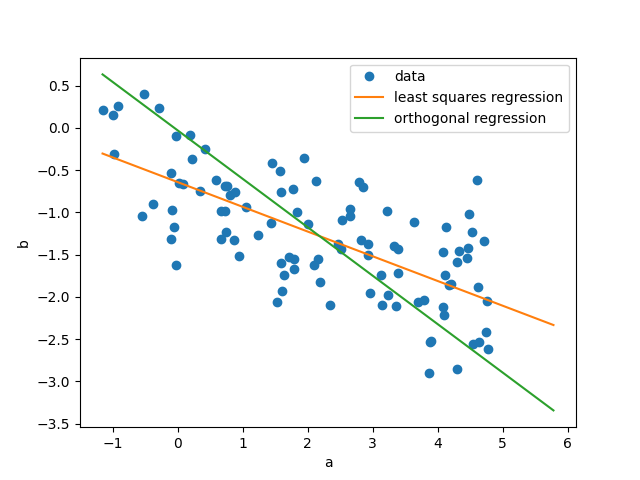
\includegraphics[scale=0.5]{test.png}
\section*{Exercise A2.4}
Expanding $(1+A)^{n-1}$, we get
$$
(1+A)^{n-1}=\sum_{k=1}^{n-1}A^k$$
Since $A^k_{i,j}$ represents whether a path of length exists from $j$ to $i$, (with $A^k_{i,j}>0$ representing that such a path exitst)
we can see that the sum of the $A^k$ matrices for $1\leq k \leq n-1$ represents all the paths that can possibly exists. Therefore $A$ is
irreducible if it possible to travel to one node to any other node, ie that $G_A$ is strongly connected.
\section*{Exercise A2.8}
We can start by multiplying each $x_i$ subvectors with $B$, each of these operations takes $(2n-1)n$ flops, so for the $n$ subvectors it will cost us $(2n-1)n^2$ flops.
\\\\Now we get that for the ith output subvector $y_i=\sum_{j=1}^{n}A_{i,j}Bx_j$. Multiplying $A{i,j}$ with $Bx_j$ costs us $n$ flops, therefore repeating this $n$ times for 
$1\leq i \leq n$ results in $n^2$ flops. Summing these vectors $A_{i,j}Bx_j$ costs $n(n-1)$ flops. So in total computing this subvector costs us $2n(n-1)$ flops. We will need to repeat this for each of the $n$ output subvectors, so it will cost use $2n^2(n-1)$.\\\\
Therefore in total, this algorithm will cost us $2n^2(n-1)+(2n-1)n^2$ flops, so approximatley $4n^3$ flops for large $n$. In comparison the algorithm for computing $(n^2,n^2)$ matrix multiplied with an $n^2$ vector will take $(2n^2-1)n^2$ flops, or $2n^4$ flops approximatley for large $n$.
\section*{Exercise A2.10}
\subsection*{(a)}
For any $k$ that satisfy $i\leq k < j$, we have that we can rearange the multiplication of $A_iA_{i+1}...A_{j}$ to $(A_i..A_k)(A_{k+1}..A_j)$.\\\\
We have that multiplying the matrices from $i$ to $k$ will cost us $c_{i,k}$ flops and result in a
matrix of size $(n_{i-1},n_k)$, likewise multiplying the matrices from $k+1$ to $j$ will cost us $c_{k+1,j}$ flops and result in a matrix of size $(n_{k},n_j)$.\\\\
Multiplying these two matrices together will cost us $2n_{i-1}n_kn_j$. Therefore if we split up the computation of 
$A_iA_{i+1}...A_{j}$ into two parts, one from $i$ to $k$ the other from $k+1$ to $j$, we will have thatv the total cost of computing $A_iA_{i+1}...A_{j}$ is:
$$c_{i,k}+c_{k+1,j}+2n_{i-1}n_kn_j$$
Therefore the minimum of the cost of computing $A_iA_{i+1}...A_{j}$ is when $k$ is the value that minimizes the above expression. In otherwords:
$$c_{i,j}=\min_{k=i,i+1,...,j-1}(c_{i,k}+c_{k+1,j}+2n_{i-1}n_kn_j)$$
\subsection*{(b)}
We have that the triangular table of $c_{i,j}$ for $A_1A_2A_3A_4$ is:
$$\begin{matrix}
    0&1.00\cdot 10^{10}&1.20\cdot 10^{10}&1.21\cdot 10^{9}&\\
    & 0&1.00\cdot 10^{11}&1.20\cdot 10^{9}&\\
    & & 0&2.00\cdot 10^{8}&\\
    & & & 0&\\
    \end{matrix}$$
Therefore the optimal cost of computing $A_1A_2A_3A_4$ 
is multiply $A_1$ with the product of $A_2$ multiplied with the product of $A_3$ and $A_4$, 
which takes us $\boxed{1.21\cdot 10^9}$ flops.
\\\\
Likewise since the triangular table of $c_{i,j}$ for $A_1A_2A_3$ is:
$$\begin{matrix}
    0&1.00\cdot 10^{10}&1.20\cdot 10^{10}&\\
    & 0&1.00\cdot 10^{11}&\\
    & & 0&\\
    \end{matrix}$$
The optimal cost of $A_1A_2A_3$ is to multiply $(A_1A_2)$ with $A_3$, 
which takes us $1.20\cdot 10^{10}$ flops. So interestingly the optimal flops
to compute $A_1A_2A_3A_4$ less than the optimal flops to compute $A_1A_2A_3$, 
despite the fact that $A_1A_2A_3A_4$ involves one more matrix multiplication. Likewise the
optimal order for the multiplication also changes when we try to compute $A_1A_2A_3A_4$ compared to $A_1A_2A_3$.

\end{document}



